\documentclass[12pt, titlepage]{article}

\usepackage{fullpage}
\usepackage[round]{natbib}
\usepackage{multirow}
\usepackage{booktabs}
\usepackage{tabularx}
\usepackage{graphicx}
\usepackage{float}
\usepackage{hyperref}
\hypersetup{
    colorlinks,
    citecolor=black,
    filecolor=black,
    linkcolor=red,
    urlcolor=blue
}
\usepackage[round]{natbib}

\newcounter{acnum}
\newcommand{\actheacnum}{AC\theacnum}
\newcommand{\acref}[1]{AC\ref{#1}}

\newcounter{ucnum}
\newcommand{\uctheucnum}{UC\theucnum}
\newcommand{\uref}[1]{UC\ref{#1}}

\newcounter{mnum}
\newcommand{\mthemnum}{M\themnum}
\newcommand{\mref}[1]{M\ref{#1}}

\title{SE 3XA3: Module Guide: Rev 1 \\Plagiarism Check}

\author{Team 310, MXQ Gang
		\\ Qifeng Xu, xuq14
		\\ Xu Wang, wangx147
		\\ Mrinal Tiwari, tiwarim
}


\date{\today}


\begin{document}

\maketitle

\pagenumbering{roman}
{
  \hypersetup{linkcolor=black}
  \tableofcontents
}
{
  \hypersetup{linkcolor=black}
  \listoftables
}

{
  \hypersetup{linkcolor=black}
  \listoffigures
}


\begin{table}[H]
\caption{\bf Revision History}
\begin{tabularx}{\textwidth}{p{3cm}p{2cm}X}
\toprule {\bf Date} & {\bf Version} & {\bf Notes}\\
\midrule
Mar 12, 2020 & 1.0 & added the Module Guide\\
\midrule
\textcolor{red}{April 6, 2020} & \textcolor{red}{1.1}& \textcolor{red}{Updated the Module Guide}\\
\bottomrule
\end{tabularx}
\end{table}

\newpage

\pagenumbering{arabic}

\section{Introduction}

\subsection{Overview}

This project is to redevelop a plagiarism checker that can detect the similarity ratio of two documents. The  purpose  of  this  software  is  to  avoid  plagiarism  for  writing  essays  and documentations.  It is able to assist students and researchers to accomplish better documents.

\subsection{Context}

This document is the Module Guide, which is created along with Module Interface Specification after the Software Requirements Specification. The purpose of the SRS document is to illustrate and explain all the functional and non-functional requirements for
the project. Based on the SRS document, the Module Guide provides a way to decompose the system into multiple modules, and describes
the modular structure. The Module Guide also documents the connection between requirements and modules in this system. Module Interface Specification will be created along with the Module Guide in order to describe the detailed semantics and syntax of each module in the system.

\subsection{Design Principles}

Decomposition needs to be guided by principles and patterns. The design principles used for decomposition of this system are information hiding, principle of low coupling and high cohesion and "fan-in" in uses relation.
The information hiding principle makes sure that each expected change is encapsulated and design interface will not change even when the module secret changes. Low coupling and high cohesion principle ensures that modules are independent and the elements in each module are strongly related.

\subsection{Document Structure}

\begin{itemize}

\item Section 2 lists possible changes to the system. According to the likeliness of the change, the possible changes are classified into two categories. Anticipated changes are listed in Section \ref{SecAchange}, and unlikely changes are listed in Section \ref{SecUchange}.

\item Section 3 provides an overview of the module design. Modules are summarized in a hierarchy decomposed by secrets in a table.

\item Section 4 provides the Connection Between Requirements and Design, which describes how the the design of the system is intended to satisfy the requirements developed in the SRS.

\item Section 5 provides the detailed Module Decomposition information. 

\item Section 6 shows two traceability matrices: between the modules and the requirements and between the modules and the anticipated changes.

\item Section 7 provides the Uses Hierarchy between modules.

\end{itemize}	

\section{Anticipated and Unlikely Changes} \label{SecChange}

\subsection{Anticipated Changes} \label{SecAchange}

Anticipated changes are the source of the information that is to be hidden
inside the modules. Ideally, changing one of the anticipated changes will only
require changing the one module that hides the associated decision. The approach
adapted here is called design for
change.

\begin{description}
\item[\refstepcounter{acnum} \actheacnum \label{acHardware}:] The specific hardware on which the software is running.

\item[\refstepcounter{acnum} \actheacnum \label{acSystem}:] The operating system on which the software is running.

\item[\refstepcounter{acnum} \actheacnum \label{acBrowser}:] The browser on which the software is running.

\item[\refstepcounter{acnum} \actheacnum \label{acLanguage}:] The language characters of text that users input.

\item[\refstepcounter{acnum} \actheacnum \label{aclength}:] The length of texts that users input.

\item[\refstepcounter{acnum} \actheacnum \label{aclength}:] The payment method for tokens.

\item[\refstepcounter{acnum} \actheacnum \label{aclength}:] UI style that might vary for different operating systems.



\end{description}

\subsection{Unlikely Changes} \label{SecUchange}

The module design should be as general as possible. However, a general system is
more complex. Sometimes this complexity is not necessary. Fixing some design
decisions at the system architecture stage can simplify the software design. If
these decision should later need to be changed, then many parts of the design
will potentially need to be modified. Hence, it is not intended that these
decisions will be changed.

\begin{description}
\item[\refstepcounter{ucnum} \uctheucnum \label{ucIO}:] Input/Output devices (Input: File and/or Keyboard, Output: File, Memory, and/or Screen).

\item[\refstepcounter{ucnum} \uctheucnum \label{ucInput}:] The format of the initial input data.

\item[\refstepcounter{ucnum} \uctheucnum \label{ucOutput}:] The format of the final output data.



\end{description}

\section{Module Hierarchy} \label{SecMH}

This section provides an overview of the module design. Modules are summarized
in a hierarchy decomposed by secrets in Table \ref{TblMH}. The modules listed
below, which are leaves in the hierarchy tree, are the modules that will
actually be implemented.

\begin{description}
\item [\refstepcounter{mnum} \mthemnum \label{mHH}:] Hardware Hiding Module

\item [\refstepcounter{mnum} \mthemnum \label{mHH}:] Register Module

\item [\refstepcounter{mnum} \mthemnum \label{mHH}:] Detect Module

\item [\refstepcounter{mnum} \mthemnum \label{mHH}:] Refill Module

\item [\refstepcounter{mnum} \mthemnum \label{mHH}:] Integration Module

\item [\refstepcounter{mnum} \mthemnum \label{mHH}:] Application Module

\item [\refstepcounter{mnum} \mthemnum \label{mHH}:] Sysutils Module

\end{description}


\begin{table}[h!]
\centering
\begin{tabular}{p{0.3\textwidth} p{0.6\textwidth}}
\toprule
\textbf{Level 1} & \textbf{Level 2}\\
\midrule

{Hardware-Hiding Module} & ~ \\
\midrule

\multirow{3}{0.3\textwidth}{Behaviour-Hiding Module} & Register Module\\
& Detect Module\\
& Refill Module\\

\midrule

\multirow{3}{0.3\textwidth}{Software Decision Module} 
& Application Module\\
& Sysutils Module\\
& Integration Module\\
\bottomrule

\end{tabular}
\caption{\bf Module Hierarchy}
\label{TblMH}
\end{table}

\section{Connection Between Requirements and Design} \label{SecConnection}

The design of the system is intended to satisfy the requirements developed in
the SRS. In this stage, the system is decomposed into modules. For the FR3 that user's password shall not be stored in database as the original password, it will be satisfied through Register Module by an encryption algorithm. This encryption mechanism also satisfies the security requirements in order to protect users' privacy. The Detect Module realizes the functional requirements 4-6 by implementing input functions and a texts comparing algorithm. The Refill Module makes sure that users can refill their tokens with a certain amount when they run out of it. 

Application Module checks which resource is getting called by the Integration Module and directs to either Register, Detect and Refill Modules. Sysutils Module provides helper functions to reduce code duplication and improve code reusability. Integration Module also realizes the look and feel requirements by implementing a user-friendly GUI. It shall make it easier for users to operate our software, therefore, it satisfies the ease of use requirements as well.

\section{Module Decomposition} \label{SecMD}

Modules are decomposed according to the principle of ``information hiding''
proposed by \citet{ParnasEtAl1984}. The \emph{Secrets} field in a module
decomposition is a brief statement of the design decision hidden by the
module. The \emph{Services} field specifies \emph{what} the module will do
without documenting \emph{how} to do it. For each module, a suggestion for the
implementing software is given under the \emph{Implemented By} title. If the
entry is \emph{OS}, this means that the module is provided by the operating
system or by standard programming language libraries.  Also indicate if the
module will be implemented specifically for the software.

Only the leaf modules in the
hierarchy have to be implemented. If a dash (\emph{--}) is shown, this means
that the module is not a leaf and will not have to be implemented. Whether or
not this module is implemented depends on the programming language
selected.

\subsection{Hardware Hiding Modules (M1)}

\begin{description}
\item[Secrets:]The implementation of virtual machine
\item[Services:]Serves as a virtual hardware used by the rest of the
  system. This module provides the interface between the hardware and the
  software. So, the system can use it to display outputs or to accept inputs.
\item[Implemented By:] Python virtual machine and Operating System
\end{description}

\subsection{Behaviour-Hiding Module}

\begin{description}
\item[Secrets:]The contents of the required behaviours.
\item[Services:]Includes programs that provide externally visible behaviour of
  the system as specified in the software requirements specification (SRS)
  documents. This module serves as a communication layer between the
  hardware-hiding module and the software decision module. The programs in this
  module will need to change if there are changes in the SRS.
\item[Implemented By:] N/A
\end{description}

\subsubsection{Register Module (M2)}

\begin{description}
\item[Secrets:]Password
\item[Services:]Register a account by a username and password
\item[Implemented By:] Python Libraries
\end{description}

\subsubsection{Detect Module (M3)}

\begin{description}
\item[Secrets:]Text input
\item[Services:]Check if username and password matched, calculate the text similarity ratio.
\item[Implemented By:] Python Libraries
\end{description}

\subsubsection{Refill Module (M4)}

\begin{description}
\item[Secrets:]Tokens
\item[Services:]Refill the tokens.
\item[Implemented By:] Python Libraries
\end{description}


\subsection{Software Decision Module}

\begin{description}
\item[Secrets:] Data Structures
\item[Services:] Provides the data structures to store the information from the application.
\item[Implemented By:] N/A
\end{description}

\subsubsection{Integration Module (M5)}
\begin{description}
\item[Secrets:] User interface
\item[Services:] UI contains the code to call backend.
\item[Implemented By:] Python Libraries
\end{description}

\subsubsection{Application Module (M6)}
\begin{description}
\item[Secrets:]Resource
\item[Services:] Check which resource is getting called by the integration module and directs to either Register, Detect, Refill
\item[Implemented By:] Python Libraries
\end{description}

\subsubsection{Sysutils Module (M7)}
\begin{description}
\item[Secrets:]Helper functions
\item[Services:]Provide helper functions to reduce code duplication and code reusability
\item[Implemented By:] Python Libraries
\end{description}


\section{Traceability Matrix} \label{SecTM}

This section shows two traceability matrices: between the modules and the
requirements and between the modules and the anticipated changes.

% the table should use mref, the requirements should be named, use something
% like fref
\begin{table}[H]
\centering
\begin{tabular}{p{0.2\textwidth} p{0.6\textwidth}}
\toprule
\textbf{Req.} & \textbf{Modules}\\
\midrule
FR1 & M2\\
FR2 & M2,M3\\
FR3 & M3\\
FR4 & M3\\
FR5 & M3,M5\\
FR6 & M3\\
FR7 & M4\\
FR8 & M1\\
\bottomrule
\end{tabular}
\caption{\bf Trace Between Functional Requirements and Modules}
\label{TblRT}
\end{table}

\begin{table}[H]
\centering
\begin{tabular}{p{0.2\textwidth} p{0.6\textwidth}}
\toprule
\textbf{Req.} & \textbf{Modules}\\
\midrule
NF1 & M5\\
NF2 & M1,M5\\
NF3 & M2,M3\\
NF4 & M1\\
NF5 & M1\\
NF6 & M1\\
NF7 & M1,M2,M3,M4,M5,M6,M7\\
NF8 & M2,M3\\
NF9 & M1,M2,M3,M4,M5,M6,M7\\
NF10 & M1\\
NF11 & M1\\
NF12 & M1\\
NF13 & M2,M3,M4\\
NF14 & M1\\
NF15 & M1\\
NF16 & M1\\
NF17 & M1\\
NF18 & M2,M3,M6,M7\\
NF19 & M2,M3\\
NF20 & M1,M2,M3,M4,M5,M6,M7\\
NF21 & M1,M2,M3,M4,M5,M6,M7\\
\bottomrule
\end{tabular}
\caption{\bf Trace Between Non-Functional Requirements and Modules}
\label{TblRT}
\end{table}

\begin{table}[H]
\centering
\begin{tabular}{p{0.2\textwidth} p{0.6\textwidth}}
\toprule
\textbf{AC} & \textbf{Modules}\\
\midrule
AC1 & M1\\
AC2 & M1\\
AC3 & M1\\
AC4 & M2,M3\\
AC5 & M2,M3\\
AC6 & M4\\
AC7 & M5\\
\bottomrule
\end{tabular}
\caption{\bf Trace Between Anticipated Changes and Modules}
\label{TblRT}
\end{table}


\section{Use Hierarchy Between Modules} \label{SecUse}

In this section, the uses hierarchy between modules is
provided. Parnas1978 said of two programs A and B that A {\em uses} B if
correct execution of B may be necessary for A to complete the task described in
its specification. That is, A {\em uses} B if there exist situations in which
the correct functioning of A depends upon the availability of a correct
implementation of B.  Figure \ref{FigUH} illustrates the use relation between
the modules. It can be seen that the graph is a directed acyclic graph
(DAG). Each level of the hierarchy offers a testable and usable subset of the
system, and modules in the higher level of the hierarchy are essentially simpler
because they use modules from the lower levels.

\begin{figure}[H]
\centering
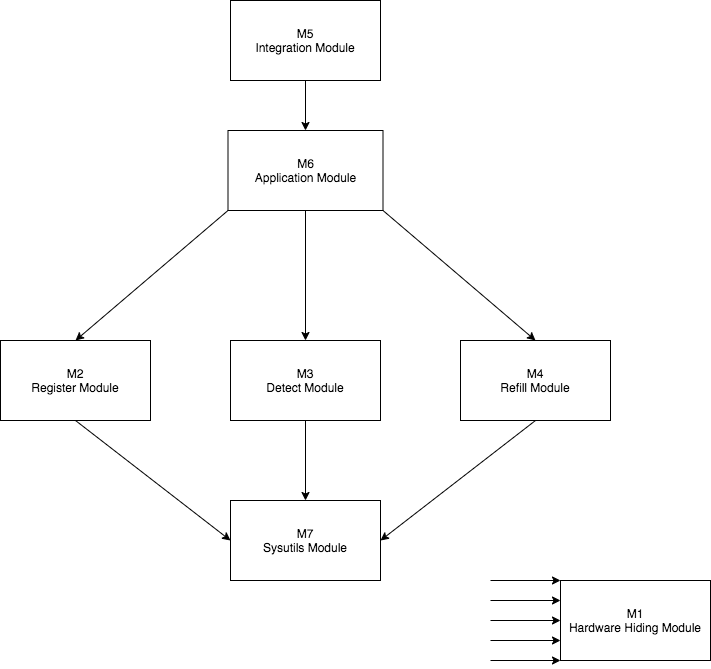
\includegraphics[width=0.7\textwidth]{UsesHierarchy.png}
\caption{\bf Use hierarchy among modules}
\label{FigUH}
\end{figure}

%\section*{References}

\bibliographystyle {plainnat}
\bibliography {MG}

\end{document}

